\section{Results}\label{sec:ex1results}
This part of the chapter provides the results of the experiment related to the established $H_0$ hypothesis as well as insights from demographical data. Data visualisation for these results is provided by SPSS due to the large data file sizes. A significance level of 0.05 was used for all statistical tests. For the sake of disclosure for any graphs that directly mention participant ID's, the author's ID is 16. 

\subsection{Rotation Detections}
As the main focus of Experiment 1 was on detection thresholds, these first few sections are dedicated to presenting the graphs over detection events for participants as they played Ensemble Retriever. Detected rotation gains are initially presented with curvature radius detections following this.

\subsubsection{Raw Rotation Detections Sample}
\begin{figure}[tbph]
    \centering
    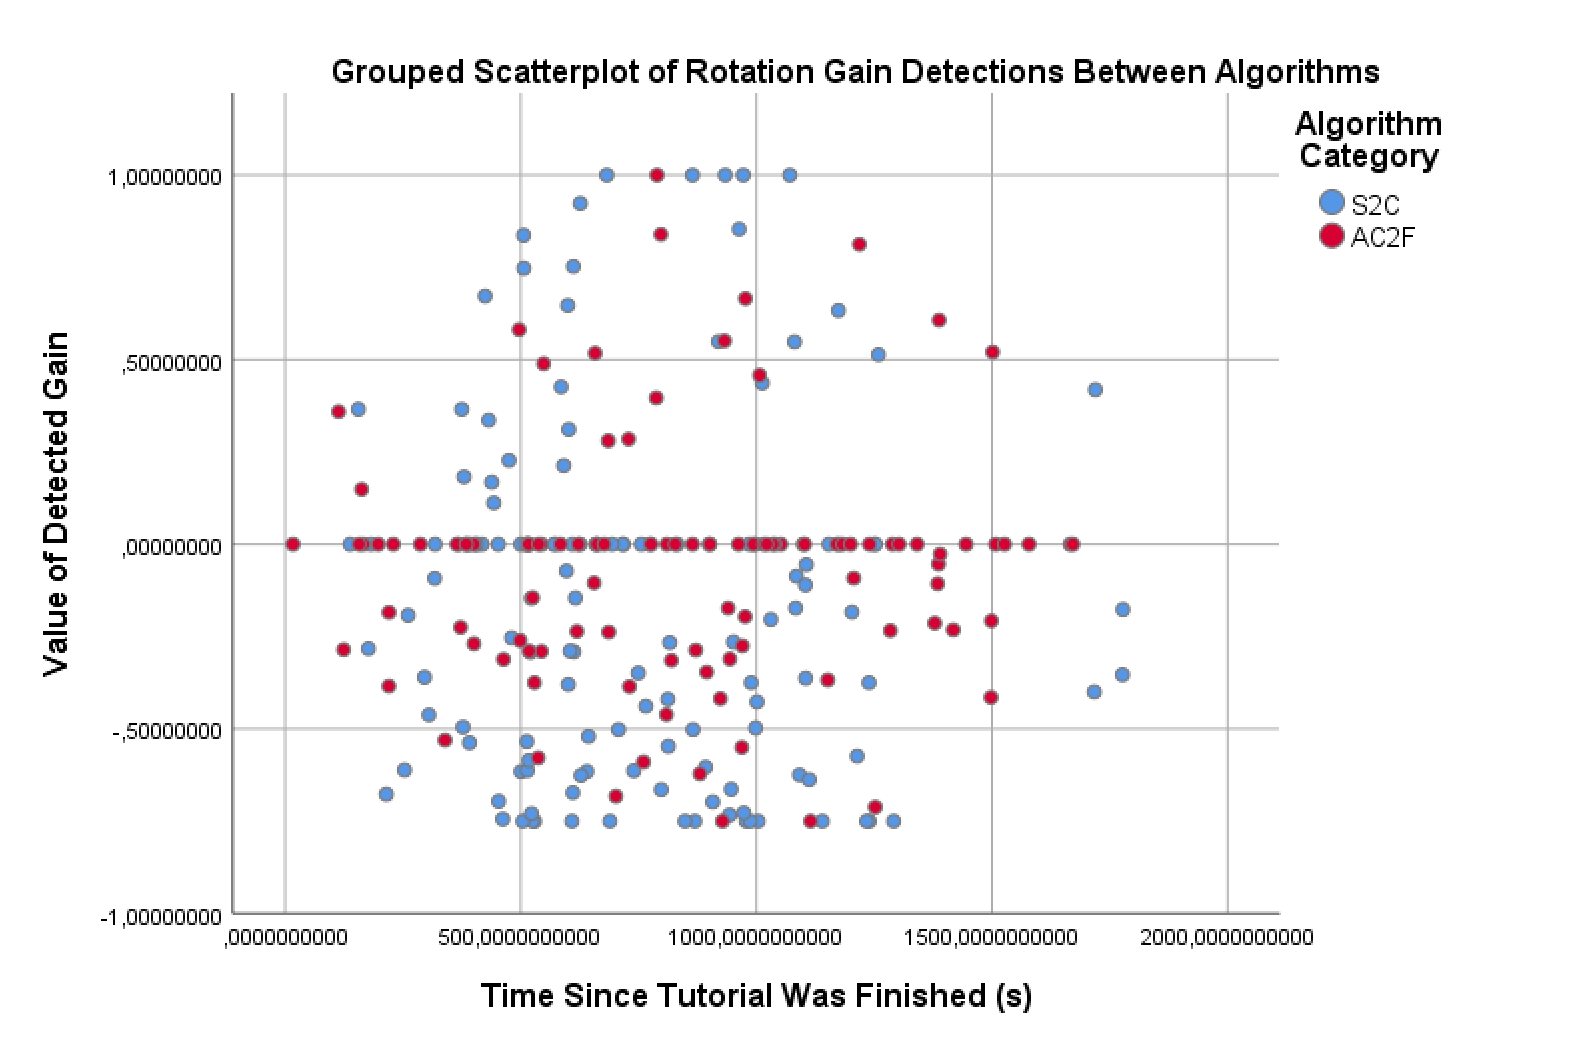
\includegraphics[width=0.75\textwidth]{figures/graphs/RawRotationDetections.png}
    \caption[Raw Detection Scatterplot For Rotation Gains]{This scatterplot shows the raw data, including outliers for rotation detections between the two employed algorithms. S2C is used for the walking state while AC2F is used for the fighting state.}
    \label{fig:rawRotationDetectionData}
\end{figure}

Before seeing the post processed sample of rotation gain detections it might be interesting to first see how the raw data looks like. This can be seen in Figure~\ref{fig:rawRotationDetectionData}. The various cases where detected gains are at a value of 0 is what the post processing step aimed to minimise. 

\subsubsection{Finalised Rotation Detections Sample}
\begin{figure}[tbph]
    \centering
    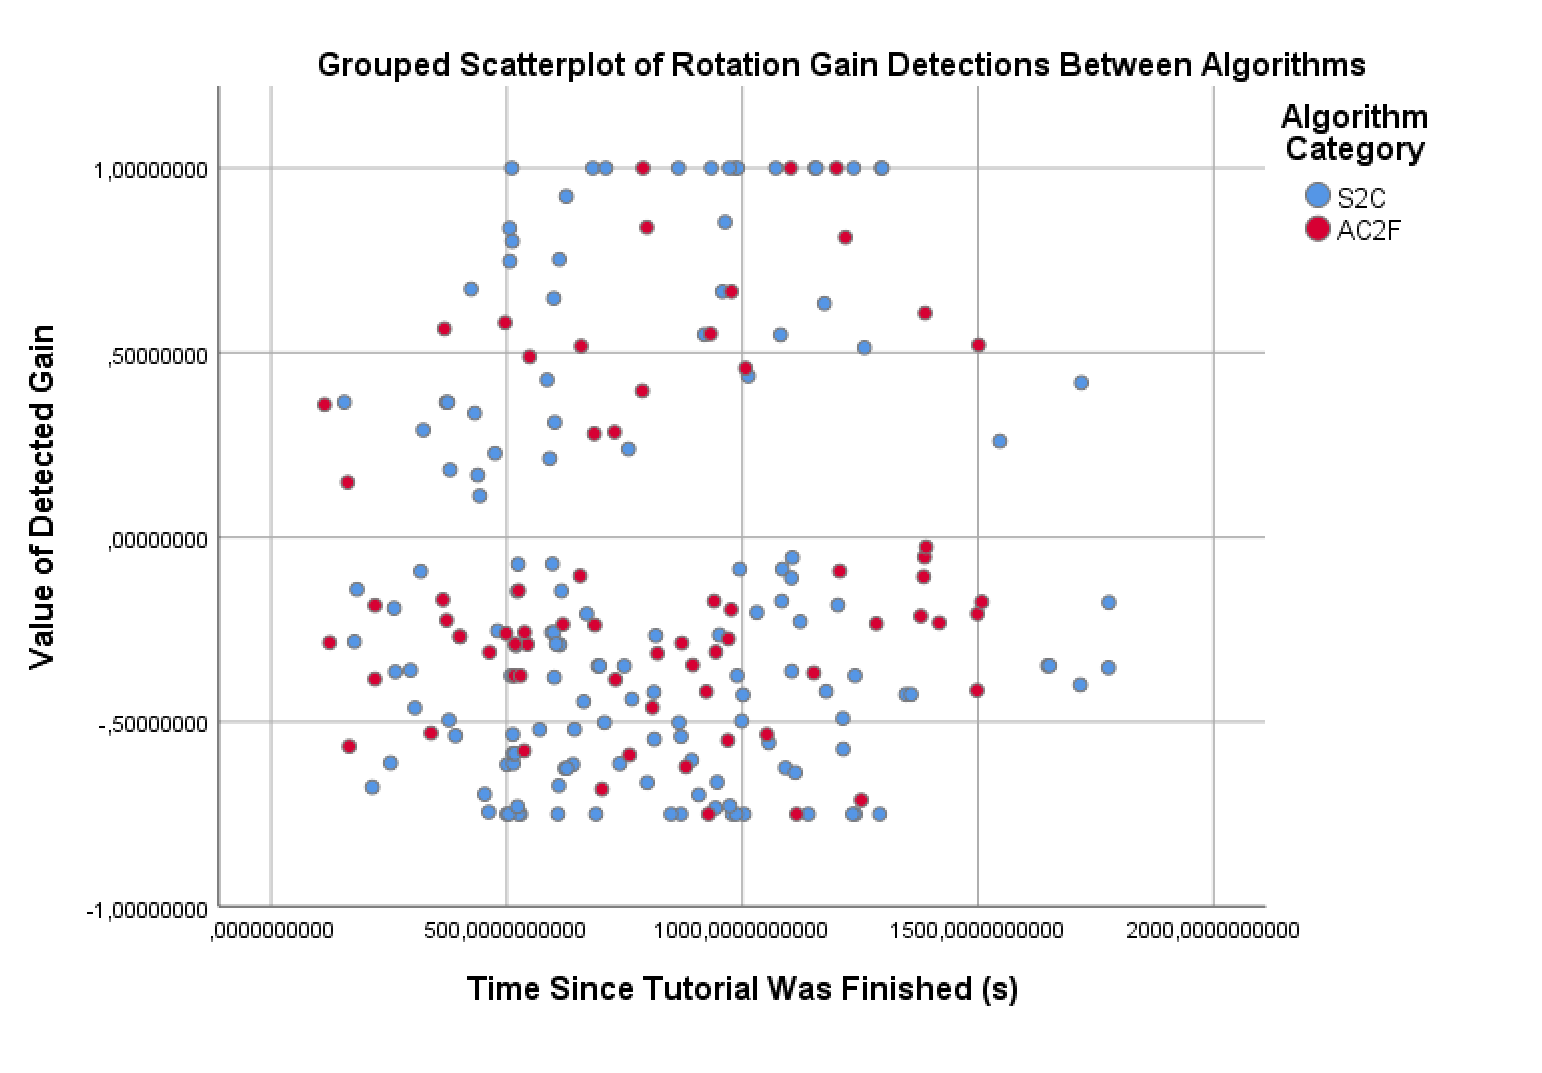
\includegraphics[width=0.75\textwidth]{figures/graphs/ProcessedRotationDetections.png}
    \caption[Finalised Detection Scatterplot For Rotation Gains, Grouped by Algorithm]{This scatterplot shows the finalised data of rotation gain detections and is grouped by algorithm.}
    \label{fig:rotationDetectionDataByAlgorithm}
\end{figure}

\begin{figure}[tbph]
    \centering
    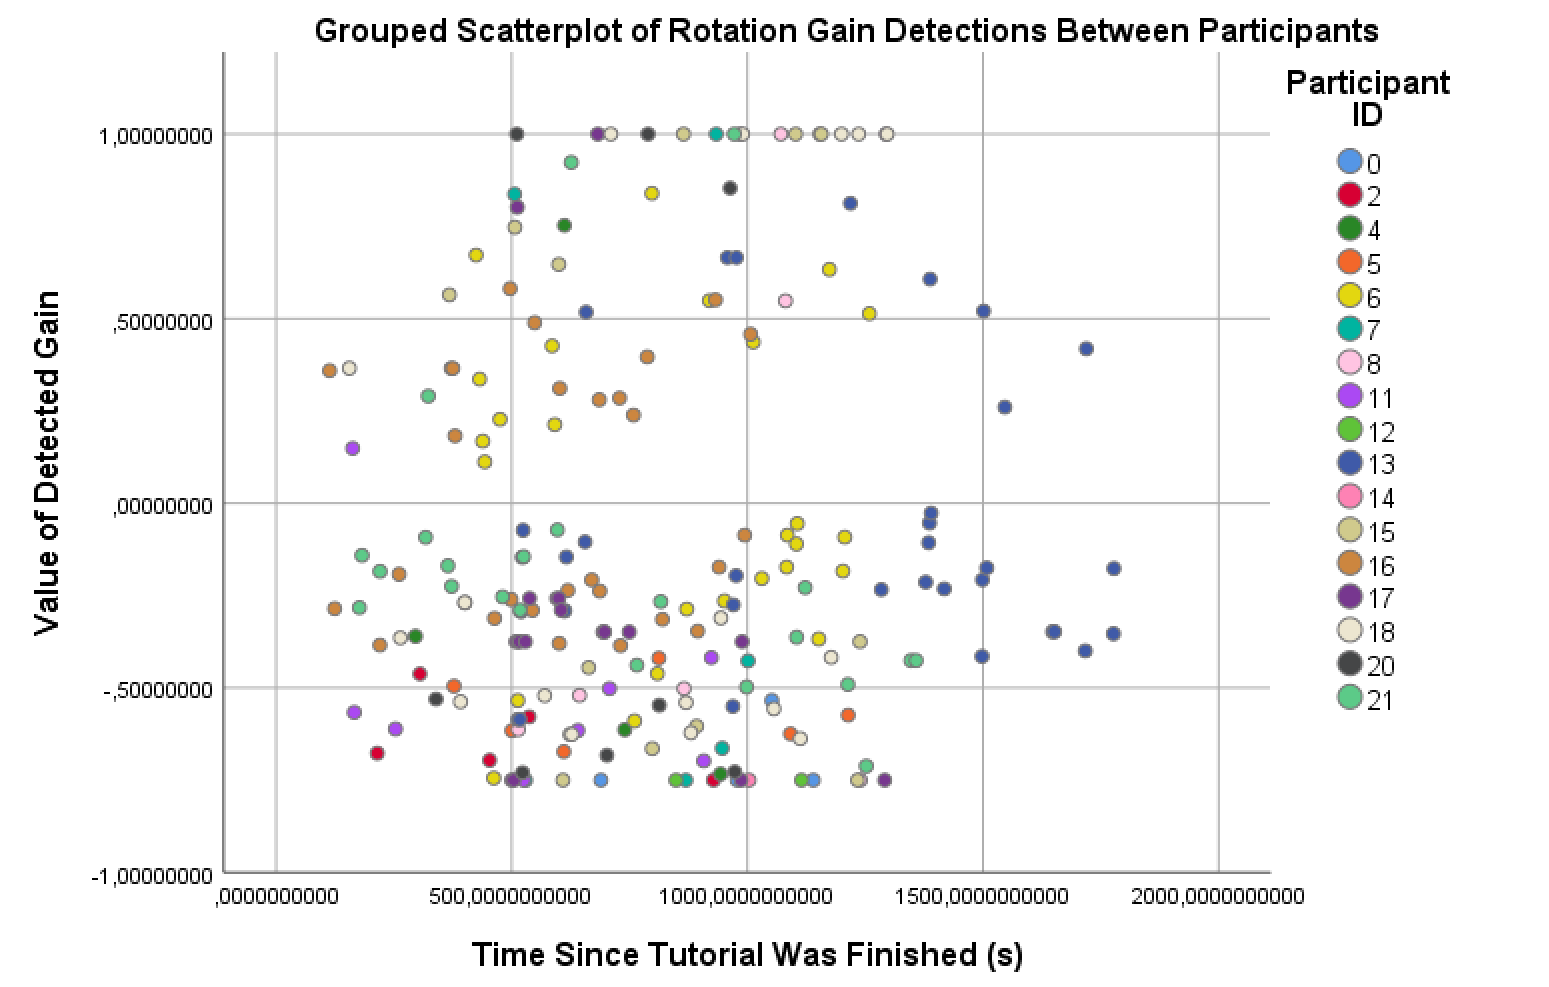
\includegraphics[width=0.75\textwidth]{figures/graphs/ProcessedRotationDetectionsByParticipant.png}
    \caption[Finalised Detection Scatterplot For Rotation Gains, Grouped by Participant ID]{This scatterplot shows the finalised data of rotation gain detections and is grouped by participant ID.}
    \label{fig:rotationDetectionDataByParticipant}
\end{figure}

\begin{figure}[tbph]
    \centering
    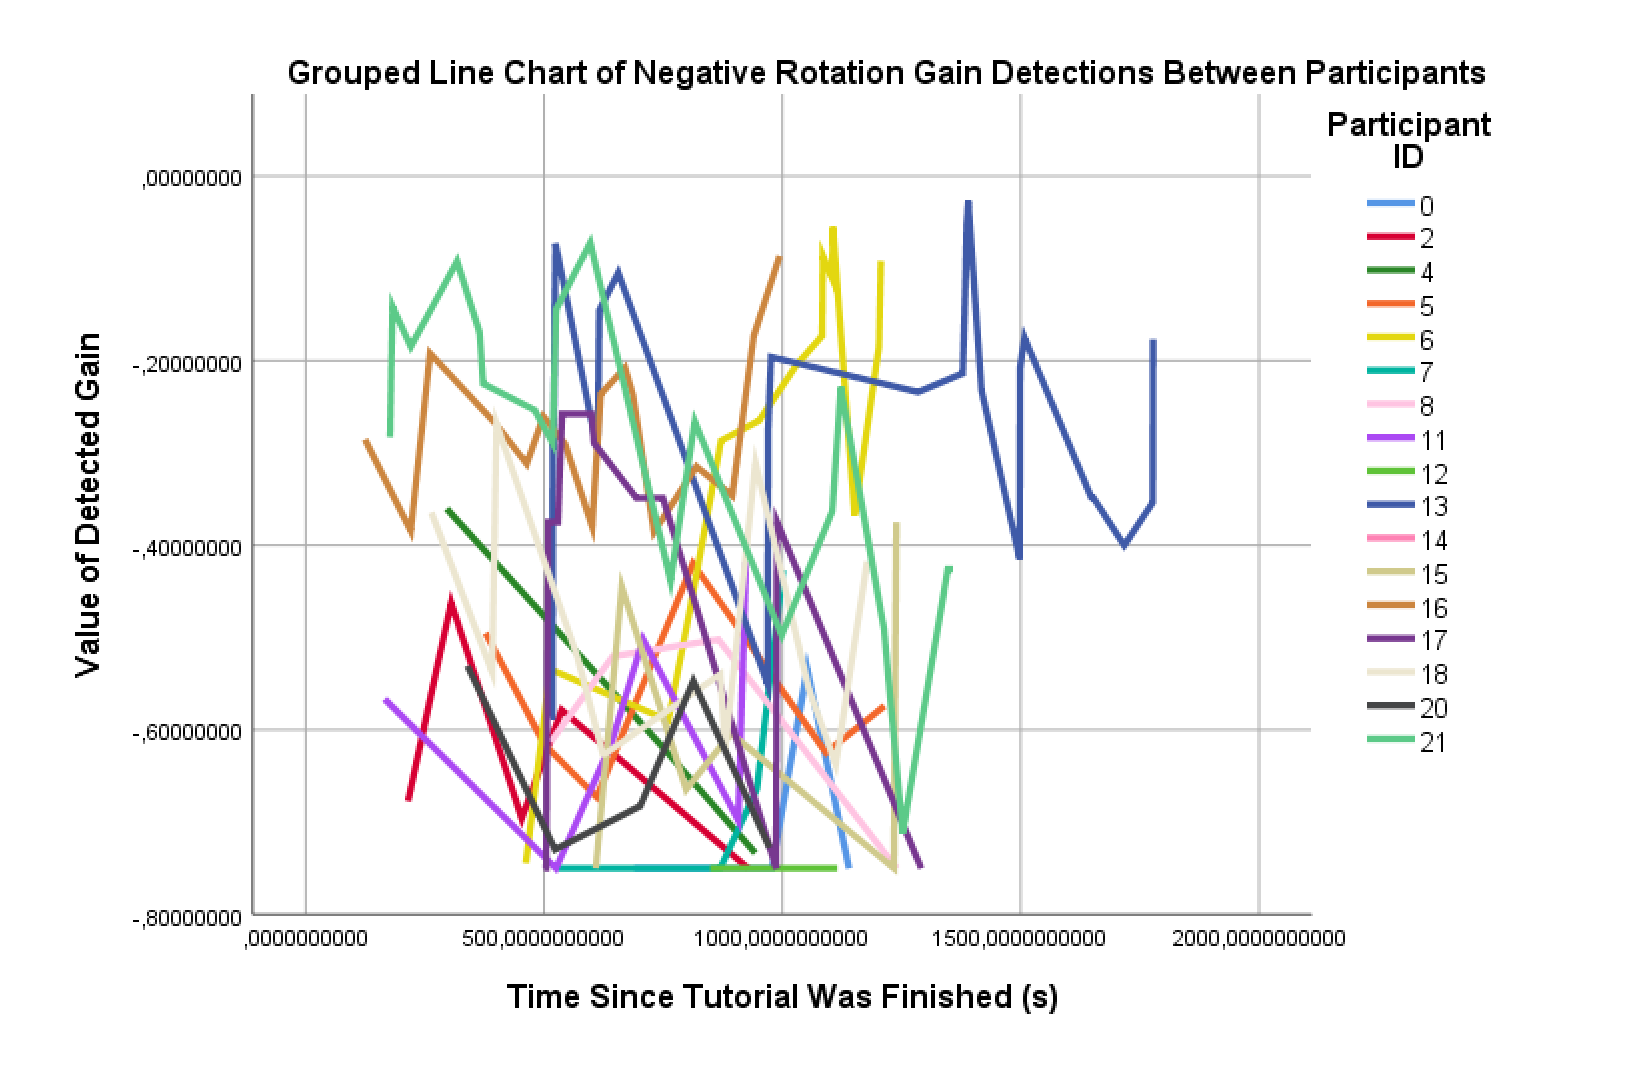
\includegraphics[width=0.75\textwidth]{figures/graphs/NegativeRotationDetectionsLineChart.png}
    \caption[Line Chart of Negative Rotation Gain Detections Between Participants]{This line chart shows the progression in negative rotation gain detections between participants.}
    \label{fig:negativeRotationDetectionLineChart}
\end{figure}

\begin{figure}[tbph]
    \centering
    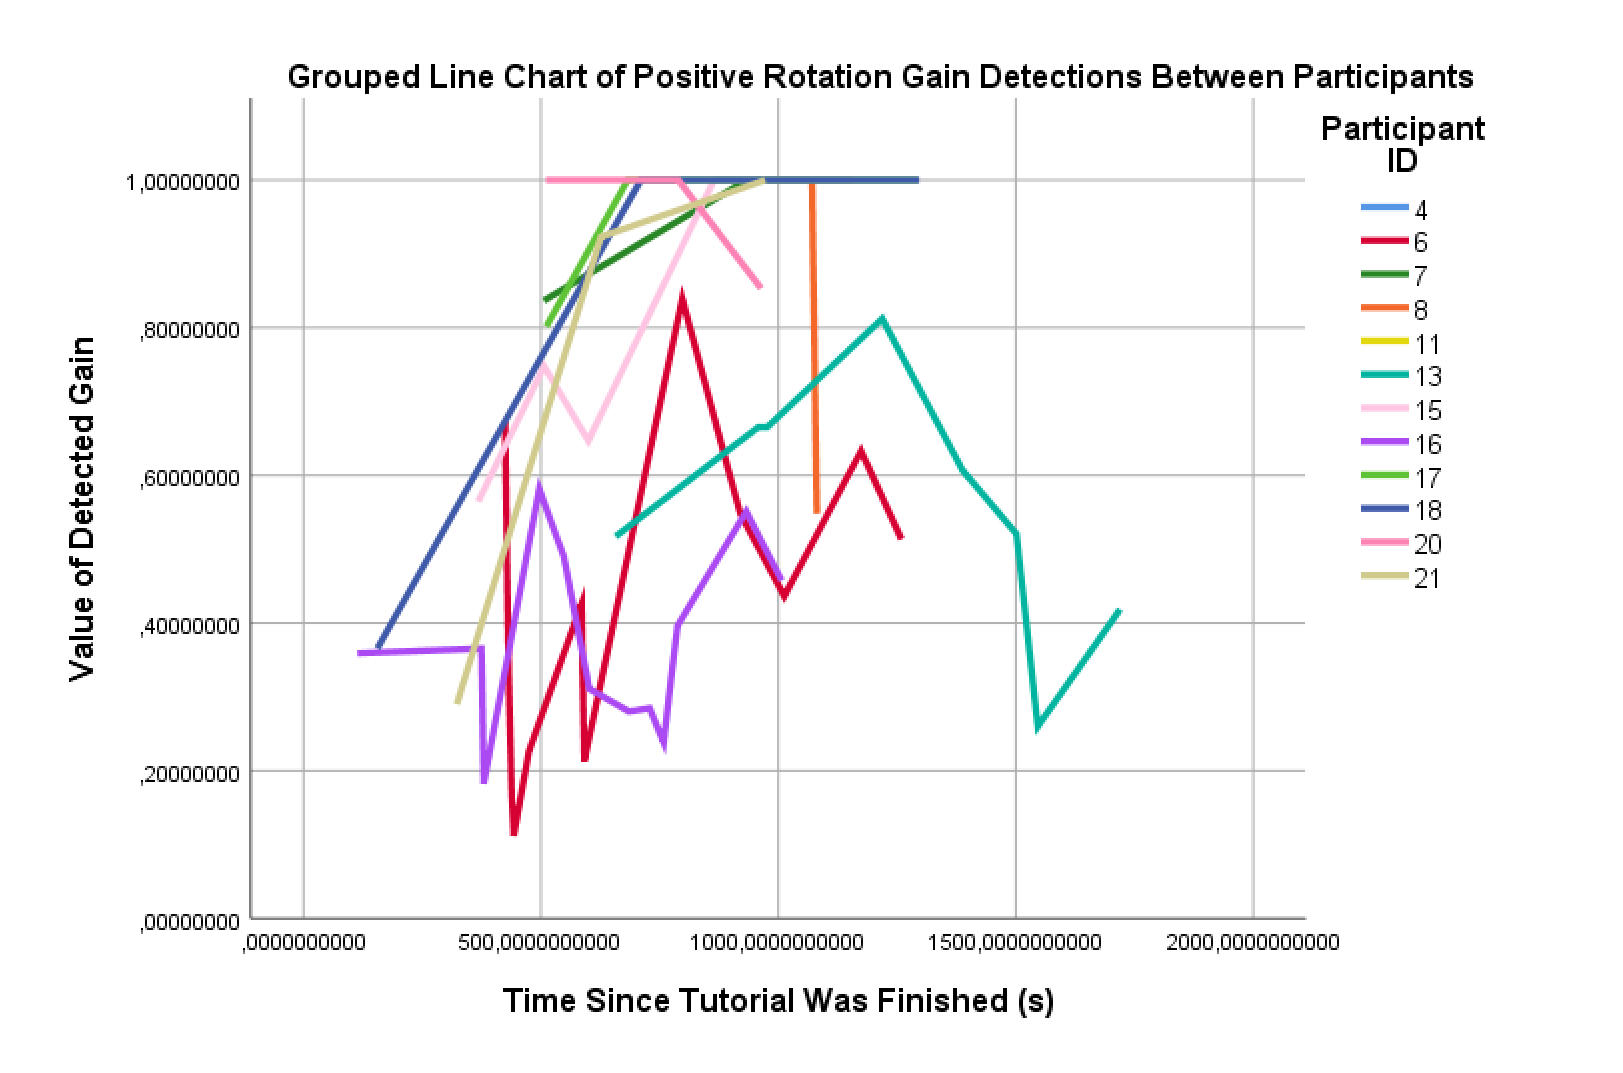
\includegraphics[width=0.75\textwidth]{figures/graphs/PositiveRotationDetectionsLineChart.png}
    \caption[Line Chart of Positive Rotation Gain Detections Between Participants]{This line chart shows the progression in positive rotation gain detections between participants.}
    \label{fig:positiveRotationDetectionLineChart}
\end{figure}

\begin{figure}[tbph]
    \centering
    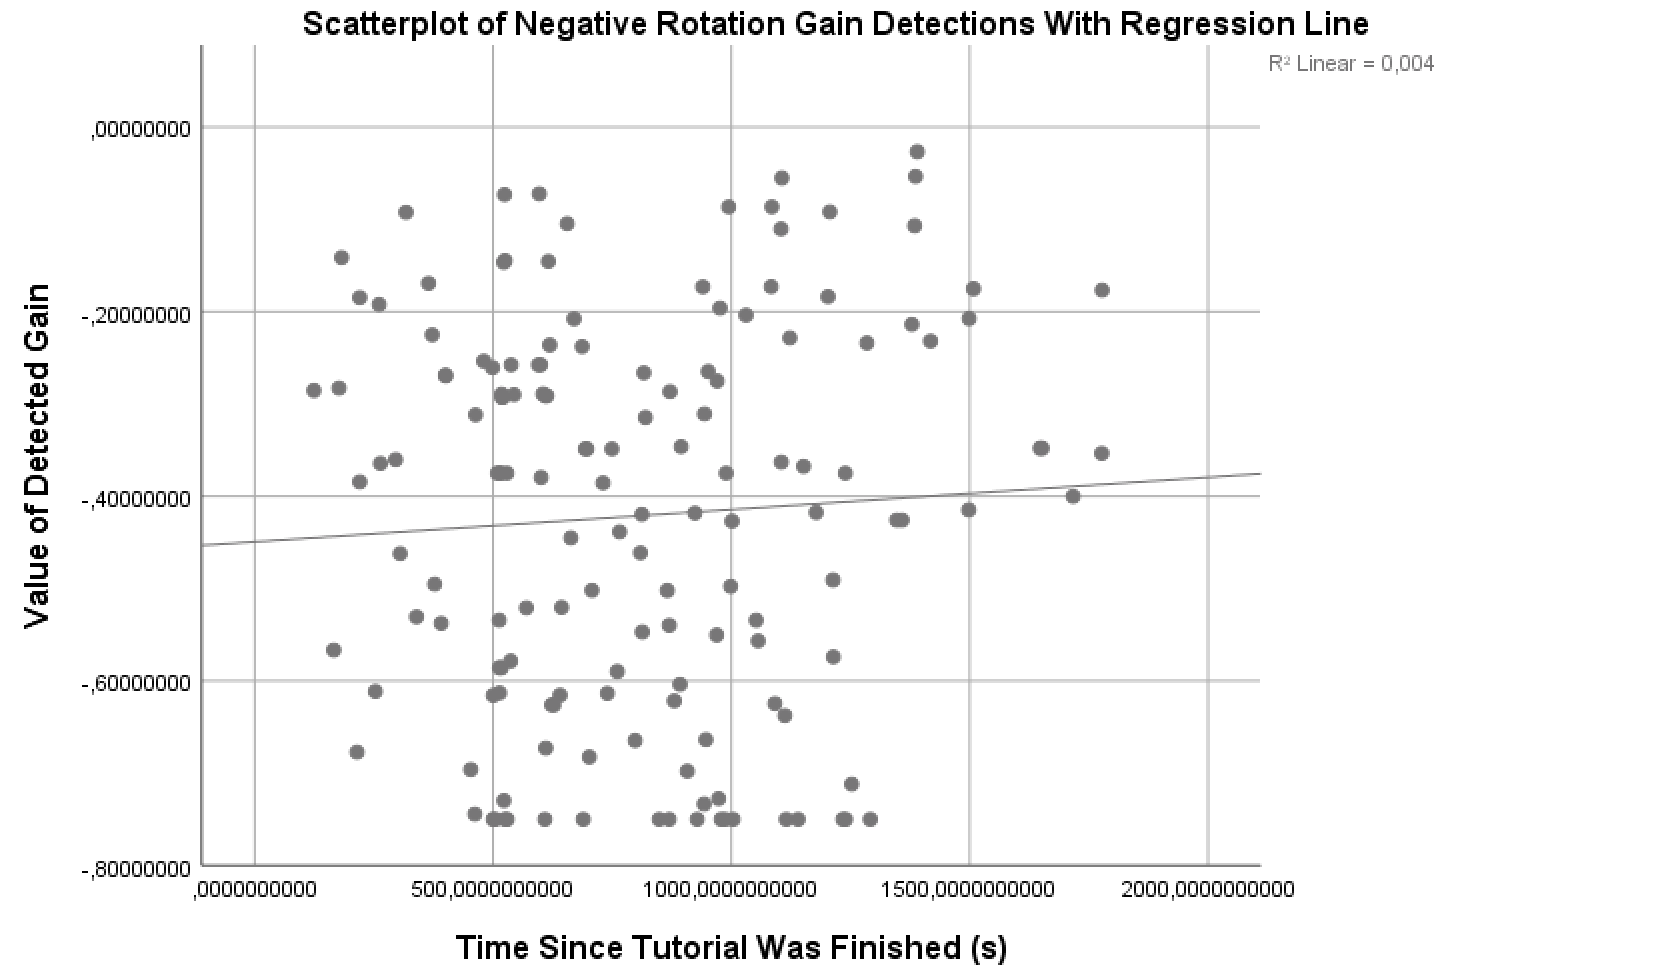
\includegraphics[width=0.75\textwidth]{figures/graphs/NegRotDetectionsRegLine.png}
    \caption[Scatterplot For Negative Rotation Gain Detections Including Regression Line]{This scatterplot shows the spread of negative rotation gain detections with an included regression line.}
    \label{fig:negRotRegLine}
\end{figure}

\begin{figure}[tbph]
    \centering
    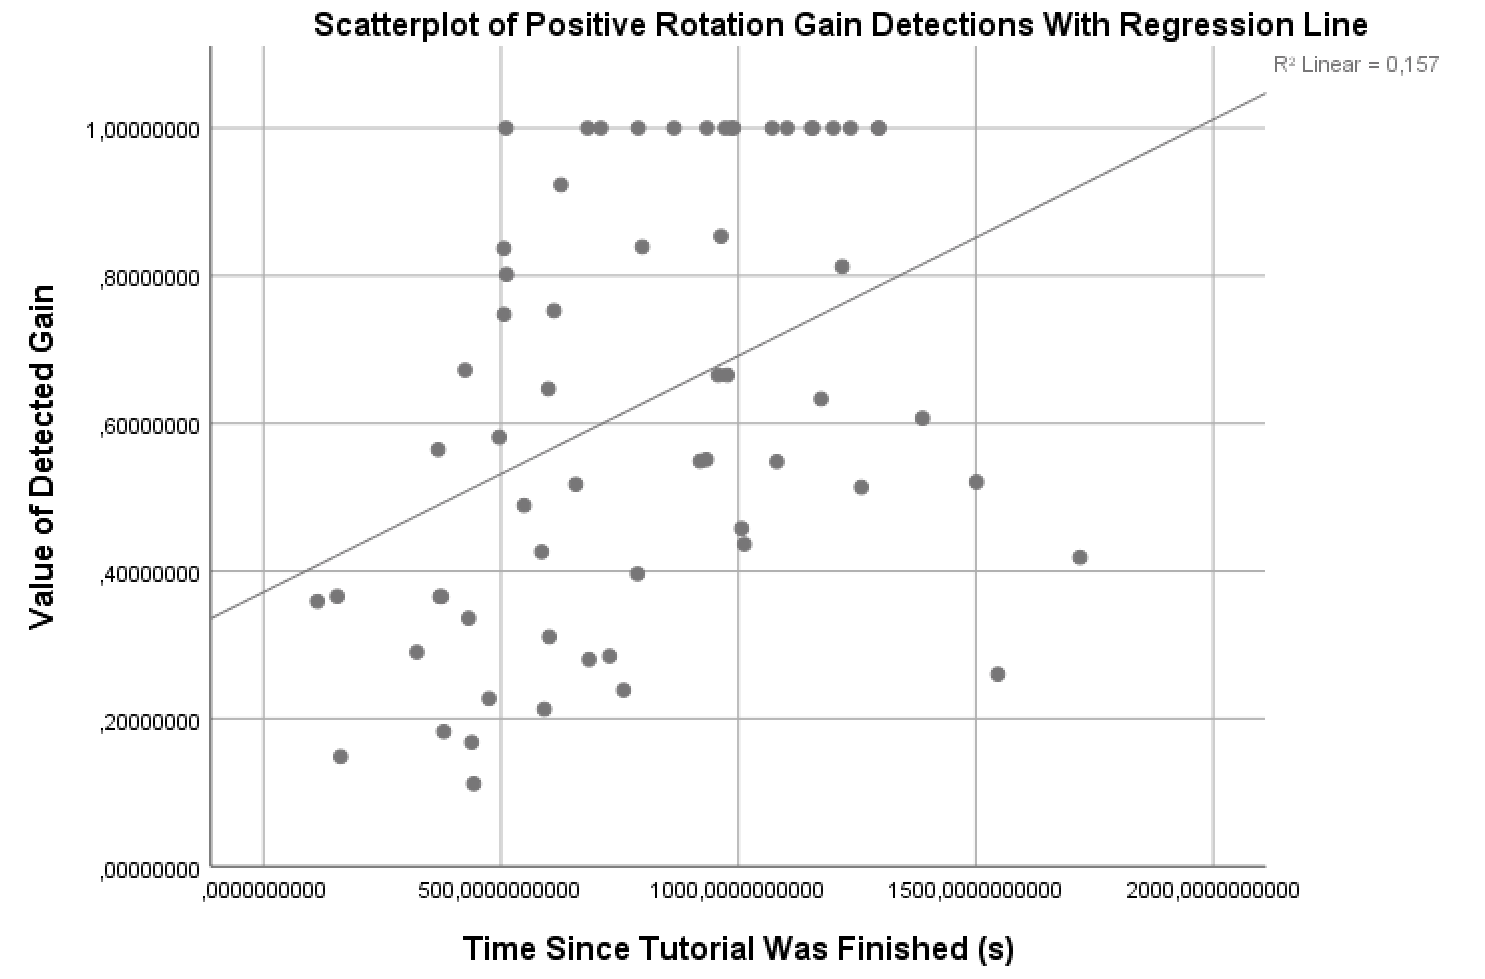
\includegraphics[width=0.75\textwidth]{figures/graphs/PosRotDetectionsRegLine.png}
    \caption[Scatterplot For Positive  Rotation Gain Detections Including Regression Line]{This scatterplot shows the spread of positive rotation gain detections with an included regression line.}
    \label{fig:posRotRegLine}
\end{figure}

\begin{figure}[tbph]
    \centering
    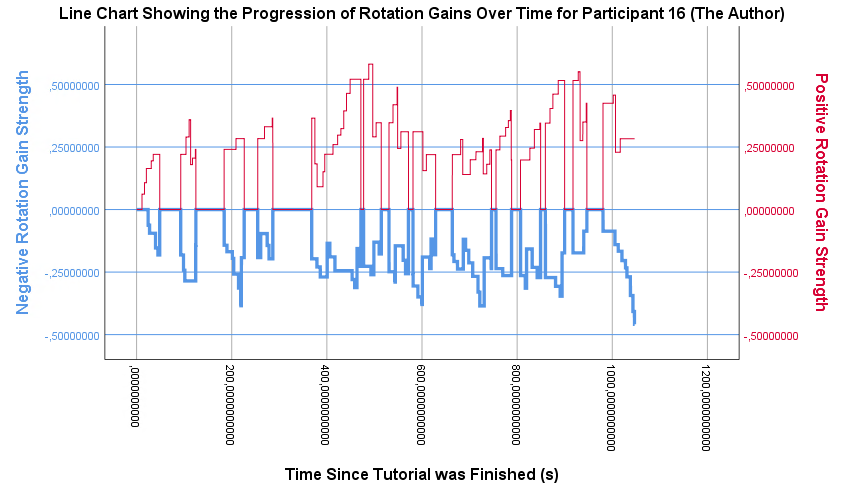
\includegraphics[width=0.75\textwidth]{figures/graphs/rotationGainProgressionAuthor.png}
    \caption[Line Chart Showing the Progression of Rotation Gains for Participant 16]{This line chart shows the progression of rotation gains over time for participant 16. Rotation gains gradually increase over time until they are detected, after which they are dropped by 50\%. Sections of time where gains are 0 are during distractor battles where the future virtual path has been aligned with the physical room centre.}
    \label{fig:authorRotationProgression}
\end{figure}

The post processing step which was mentioned in Section~\ref{sec:ex1postprocessing} resulted in 52 additional rotation gain detection events. This results in a total of 213 rotation gain detections throughout the entire sample. The processed data can be seen in Figure~\ref{fig:rotationDetectionDataByAlgorithm}, where it is grouped by algorithm and Figure~\ref{fig:rotationDetectionDataByParticipant}, where it is grouped by participant ID. To provide some additional visualisation, a line chart showing the progression of detections between participants can be seen in Figure~\ref{fig:negativeRotationDetectionLineChart} and Figure~\ref{fig:positiveRotationDetectionLineChart}.

 A figure illustrating the incremental progression of rotation gains over time for participant 16 (the author) can be seen in Figure~\ref{fig:authorRotationProgression}. Finally, individual scatterplots for negative/positive rotation gain detections with an included regression line can be found in Figure~\ref{fig:negRotRegLine} and Figure~\ref{fig:posRotRegLine}. It should be noted that some participants are not shown in these graphs as they did not provide any detection events. 

\subsection{Curvature Detections}
\begin{figure}[tbph]
    \centering
    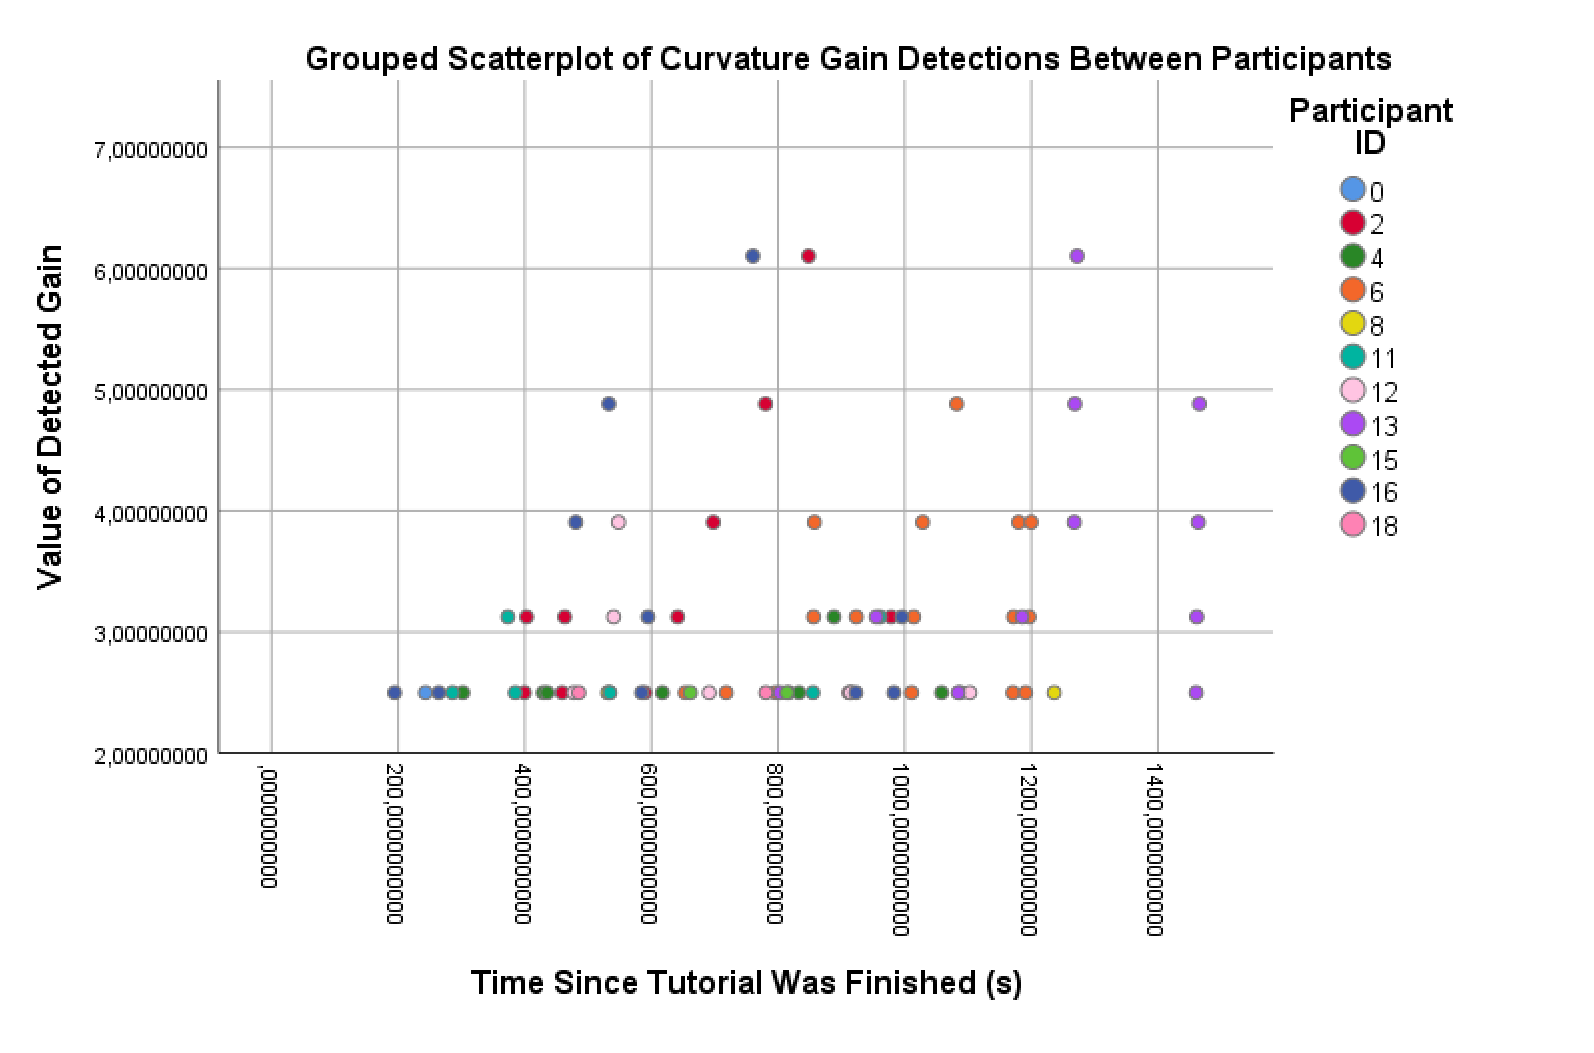
\includegraphics[width=0.75\textwidth]{figures/graphs/CurvatureDetectionScatter.png}
    \caption[Finalised Detection Scatterplot For Curvature Gains, Grouped by Participant ID]{This scatterplot shows the finalised data of curvature gain detections and is grouped by participant ID. Curvature values in this case are defined as the radius of the curvature arc.}
    \label{fig:curvatureDetectionData}
\end{figure}

The various curvature gain detection events that happened during the walking phase of Ensemble Retriever can be seen in Figure~\ref{fig:curvatureDetectionData}.

\subsection{Mean Detection Thresholds}
\begin{table}[!h]
\centering
\begin{tabularx}{\textwidth}{|X|X|}
\hline
Type of Gain & Mean Detection Threshold (N = Total Number of Detections) \\
\hline
S2C: Positive Rotation Gain & 0.6479 (N = 43) \\
\hline
S2C: Negative Rotation Gain & -0.4631 (N = 101) \\
\hline
AC2F: Positive Rotation Gain & 0.5828 (N = 19) \\
\hline
AC2F: Negative Rotation Gain & -0.3365 (N = 50) \\
\hline
Combined S2C+AC2F: Positive Rotation Gain & 0.6279 (N = 43+19) \\
\hline
Combined S2C+AC2F: Negative Rotation Gain & -0.4212 (N = 101+50) \\
\hline
S2C: Curvature Radius & 3.0978m (N = 78) \\
\hline
\end{tabularx}
\caption[Experiment 1: Mean Detection Thresholds]{This table shows the various detection thresholds that were calculated as the mean of all detection events in each respective category.}
\label{table:ex1DetectionThresholds}
\end{table}

The aggregated mean detection thresholds which have been generated out of the previously presented data can be seen in Table~\ref{table:ex1DetectionThresholds}. 

\subsection{Test for Normality}
*(Kinda methods)
   * Before deciding what statistical test to use for comparisons between Walking/Fighting conditions a test for normal distribution was used first
   * As the dataset of detections for each gain is below 2000 elements, the Shapiro-Wilk test has been used for this

Shapiro-Wilk Test:
   * Pos Rot Detections
      * p < 0.001 for the S2C Category, while a p value of 0.295 for AC2F. S2C is thus not normally distributed while AC2F is
   * Neg Rot Detections
      * p < 0.001 for S2C, while a p = 0.015 for AC2F. Both are not normally distributed
      
   * Curvature Detections
      * (Not really relevant as there is no comparisons to do with curvature gains)

Since the data is not normally distributed, it is not possible to use standard tests like the independent samples t-test.
   
\subsection{Hypothesis Testing}
* Significance level of 0.05

* Shape test before doing Mann-Whitney U:
   * Negative Rot Gains do not have what I would consider a similar shape between S2C/AC2F
   * Positive Rot Gains do not have what I would consider a similar shape between S2C/AC2F either
   * Present figures of this
* Independent observations is not a thing either. Each participant provides data in both groups. 
* Meaning I would violate two of the assumptions for the MWU test if I used it.
* Ultimately, MWU still ends up being used, but it should be noted that the power of it is decreased as a result. 

* Mann-Whitney-U test is the best fit as data is not normally distributed
   * BUT: Assumption 3 from \url{https://statistics.laerd.com/spss-tutorials/mann-whitney-u-test-using-spss-statistics.php} is violated as each participant is in both groups. It is ultimately impossible to have participants split between these two groups. 

* Since the shape of the distributed data is different, the comparison in this case will be on mean ranks. 

* Positive Rotation Gain Comparison
   * No significant difference between S2C and AC2F: (U = 362.5, p = 0.478)
* Negative Rotation Gain Comparison
   * S2C mean detection threshold goes significantly lower than AC2F (U = 1639, p < 0.001)
   
* Positive Rot Threshold
   * Due to no significant differences, this is calculated as the mean of all positive detections
   
* Negative Rot Threshold
   * While there was a significant difference, the large variability of the detections makes it very hard to conclude how accurate the detection thresholds would be. It might therefore be safer to estimate this threshold as the lower bounded mean for AC2F.

\subsection{Demographic Insights}
* Testing correlation between demographical data and the sample of detected rotation gains
   * Primarily because the curvature gain data is not worth comparing due to how most participants first noticed it at 2.5 then clicked until they stopped noticing. 
* Spearman's rho used instead of pearson as the detection data is not fully normally distributed
* Correlation matrix can be seen in Figure~\ref{fig:ex1demogcorrelationmatrix}

\begin{figure}[tbph]
    \centering
    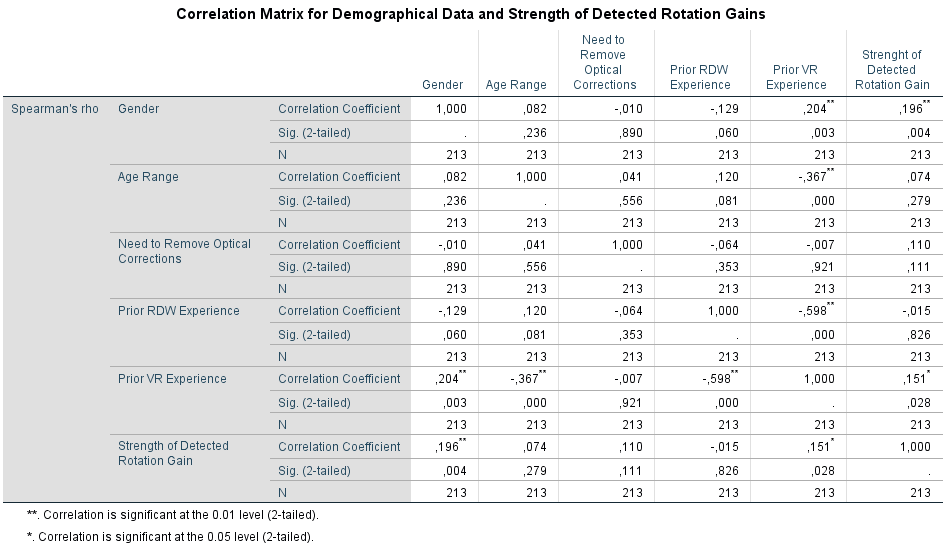
\includegraphics[width=0.8\textwidth]{figures/graphs/DemographicalCorrelations.png}
    \caption[Experiment 1 Demographical Correlation Matrix]{Correlation matrix for the demographical data in experiment 1 and the rotation gains that were detected. N values are 213 as there were 213 rotation gain detections.}
    \label{fig:ex1demogcorrelationmatrix}
\end{figure}

* Mention significant correlations

\subsubsection{Prior VR Experience and Rotation Gain Detections}
* Look deeper at Prior VR Experience


\subsubsection{Qualitative Feedback}

\subsection{Summary}
\begin{table}[h!]
\centering
\begin{tabularx}{\textwidth}{|X|X|}
\hline
Variable & Context \\
\hline
Size + Shape of Physical Tracking Space & 5m x 5.75m rectangle \\
\hline
Optical Flow/Visual Density in VE & Low Poly Artstyle. Limited visual density outside of environmental trees and shining mushrooms. The walkable environment is fully open though. The player has to fight enemy distractors while exploring which move around the player and shoot various salient projectiles that might contribute to increased optical flow and visual density. See figures in Chapter~\ref{chap:implementation} for examples.\\
\hline
Hardware: HMD Field of View & HTC Vive. ~145 diagonal degrees FoV. \\
\hline
Speed of Walking & \textasciitilde$0.2576$ $m/s$ on average (Total distance travelled / Total time spent walking between participants). Static curvature gains employed. \\
\hline
Engagement/Distraction & The participants played through a VR game which consisted of walking around, collecting clues (working memory task) and fighting enemy distractors while exploring. General engagement levels based on feedback and observation of participants could be considered as high. \\
\hline
Awareness of Redirection & Participants were informed of redirection and the basics of redirected walking. The concept of distractors was not directly explained, but mentioned in the information/consent sheet. \\
\hline
Gender & 20M, 2F \\
\hline
Estimation Method & Incrementally and randomly increasing one gain at random timesteps. Rotation gain is halved when detected, curvature radius is multiplied by 25\% when detected. \\
\hline
Adaptation: Curvature Gains & The experiment employed a incremental gains method for estimation. Gains would as such gradually increase over time. Some adaptation could be possible, but the curvature detection data cannot answer this. \\
\hline
Adaptation: Positive Rotation Gains & The data does appear to point towards a potential adaptation towards positive rotation gains. The variability of negative rotation gain detections makes it hard to say whether this also is true for these. \\
\hline
\end{tabularx}
\caption[Experiment 1: Summary Over Contextual Variables in Relation To Detection Thresholds]{Summary of variables from Chapter~\ref{chap:relatedWork} with some additions and how Experiment 1 relates to these.}
\label{table:ex1VariableSummary}
\end{table}

* A contextual summary of how the various variables from Chapter~\ref{chap:relatedWork} relate to this experiment can be found in Table~\ref{table:ex1VariableSummary}. It also includes some potentially new and relevant variables based on the results that have been shown. \todo{Estimation Method and Pos Rot Adaptation are new in this case. Might eventually just move estimation method as a variable to related work and mention how Bjørn made use of both incremental gains and regular 2AFC method.}